\section{Taxonomy and Landscape Overview}
\label{sec:taxonomy}

To organize the rapid proliferation of temporal foundation models and large language model adaptations, we present an orthogonal multi-dimensional taxonomy. As illustrated in Figure~\ref{fig:taxonomy_overview}, the landscape is structured along five fundamental axes: (1) Core Paradigm, (2) Architectural Backbone, (3) Temporal Tokenization, (4) Prediction Head \& Uncertainty, and (5) Operational Scope \& Tasks.

\begin{figure*}[t]
\centering
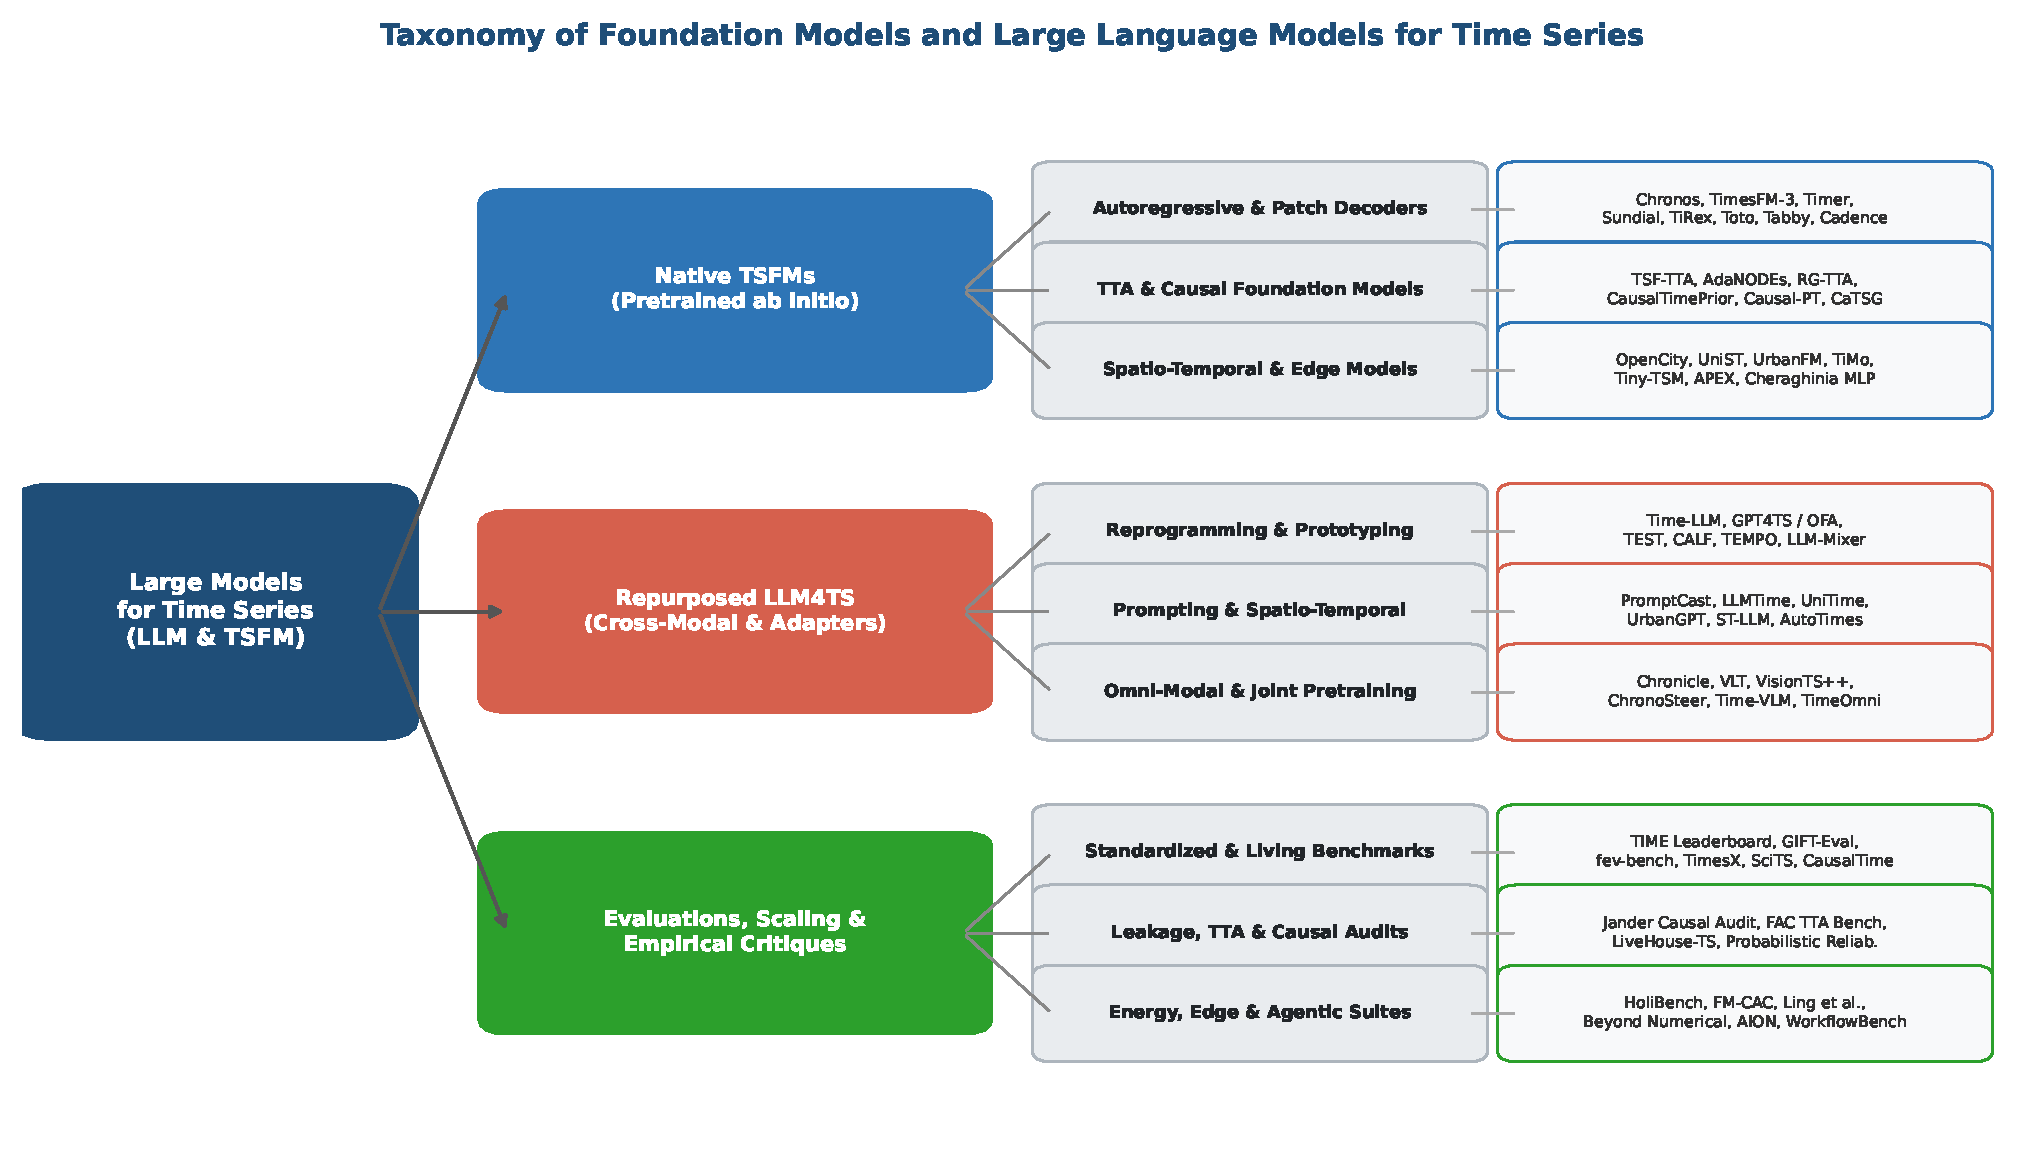
\includegraphics[width=0.98\textwidth]{figures/fig_taxonomy.pdf}
\caption{Comprehensive taxonomy of foundation models and large language models for time series, illustrating core paradigms, architectural backbones, tokenization mechanics, and representative models.}
\label{fig:taxonomy_overview}
\end{figure*}

\subsection{Taxonomy Dimensions}

\subsubsection{Dimension 1: Core Paradigm}
\begin{itemize}[leftmargin=*]
    \item \emph{Native Time Series Foundation Models (Native TSFMs)}: Models built from scratch and trained directly on large-scale collections of empirical or synthetic time-series data. Weights and latent dimensions are optimized specifically for temporal signals without textual preconceptions (e.g., Chronos~\cite{ansari2024chronos}, TimesFM~\cite{das2024timesfm}, MOIRAI~\cite{woo2024moirai}, ForecastPFN~\cite{dooley2023forecastpfn}, TiRex~\cite{auer2025tirex}, FLAME~\cite{wu2025flame}, $t_0$~\cite{meyer2026t0}).
    \item \emph{Repurposed Large Language Models (LLM4TS)}: Models that adopt pre-existing weights from language or vision transformers (e.g., Llama-2/3, GPT-2, CLIP), bridging continuous temporal modalities into text or visual embedding space via reprogramming layers, prompt prefixes, or cross-attention adapters (e.g., Time-LLM~\cite{jin2023timellm}, GPT4TS~\cite{zhou2023onefitsall}, TEST~\cite{sun2023test}, CALF~\cite{liu2024calf}, UniTime~\cite{liu2024unitime}, VisionTS~\cite{chen2024visionts}, Time-VLM~\cite{zhong2025timevlm}).
    \item \emph{Evaluation Frameworks and Benchmark Audits}: Standardized benchmarking suites and diagnostic harnesses that audit generalization, cross-domain transfer, and benchmark contamination (e.g., GIFT-Eval~\cite{salesforce2024gifteval}, SciTS~\cite{wu2025scits}, Insight Miner~\cite{zhang2025insightminer}, Time-MMD~\cite{yue2024timemmd}).
\end{itemize}

\subsubsection{Dimension 2: Architectural Backbone}
\begin{itemize}[leftmargin=*]
    \item \emph{Decoder-Only Autoregressive Transformers}: Optimized for sequential next-token or next-patch generation (e.g., TimesFM~\cite{das2024timesfm}, Timer~\cite{liu2024timer}, Chronos~\cite{ansari2024chronos}, Sundial~\cite{thuml2025sundial}, $t_0$~\cite{meyer2026t0}).
    \item \emph{Masked Encoder Transformers}: Optimized for bidirectional temporal representations via masked autoencoding (e.g., MOMENT~\cite{goswami2024moment}, PatchTST~\cite{nie2023patchtst}, VisionTS~\cite{chen2024visionts}).
    \item \emph{Encoder-Decoder Transformers}: Decoupling context representation from horizon generation (e.g., MOIRAI~\cite{woo2024moirai}, TTM~\cite{ekambaram2024ttm}, UniTS~\cite{zhou2024units}).
    \item \emph{Sparse Mixture-of-Experts (MoE)}: Dynamically routing tokens to specialized feed-forward experts to scale model capacity while maintaining constant inference FLOPs (e.g., Time-MoE~\cite{shi2024timemoe}, Moirai-MoE~\cite{woo2024moiraimoe}, Timer-S1~\cite{thuml2026timers1}).
    \item \emph{Continuous Flow and Legendre Memory Networks}: Employing continuous neural ODEs or orthogonal polynomial bases to preserve multi-scale memory (e.g., FLAME~\cite{wu2025flame}, FlowState~\cite{king2025flowstate}).
\end{itemize}

\subsubsection{Dimension 3: Temporal Tokenization}
\begin{itemize}[leftmargin=*]
    \item \emph{Uniform Subseries Patching}: Continuous linear projection of non-overlapping or strided time-step windows into dense embedding space (e.g., PatchTST~\cite{nie2023patchtst}, Timer~\cite{liu2024timer}).
    \item \emph{Scalar Discretization / Binning}: Quantizing scaled continuous observations into finite categorical tokens, allowing standard NLP cross-entropy training (Chronos~\cite{ansari2024chronos}).
    \item \emph{Decimal String Tokenization}: Casting continuous numbers into ASCII strings (e.g., ``12.4''), processed directly by off-the-shelf text tokenizers (PromptCast~\cite{xue2022promptcast}, LLMTime~\cite{gruver2023llmtime}).
    \item \emph{Multi-Resolution and Multiscale Mixing}: Dynamically decomposing and mixing patches across frequencies to resolve multi-scale seasonalities (TimeMixer~\cite{wang2024timemixer}, TimeMixer++~\cite{wang2024timemixerplus}, TTM~\cite{ekambaram2024ttm}).
    \item \emph{Visual Rendering Tokenization}: Rendering 1D numerical trajectories into 2D pixel line plots for visual encoders (VisionTS~\cite{chen2024visionts}, Time-VLM~\cite{zhong2025timevlm}).
\end{itemize}

\subsubsection{Dimension 4: Prediction Head and Uncertainty}
\begin{itemize}[leftmargin=*]
    \item \emph{Categorical Probability Distribution}: Non-parametric probability vectors over quantized bins (Chronos~\cite{ansari2024chronos}).
    \item \emph{Parametric Mixture Heads}: Estimating parameters $(\mu, \sigma, \nu)$ of explicit probability densities, such as Student's $t$ or Gaussian mixtures (Lag-Llama~\cite{rasul2023lagllama}, MOIRAI~\cite{woo2024moirai}).
    \item \emph{Deterministic Mean Squared Regression}: Direct linear or MLP projection minimizing mean squared or absolute error.
    \item \emph{Continuous Flow Matching and Diffusion}: Formulating generation as an equivariant continuous-time velocity field (FlowState~\cite{king2025flowstate}, FLAME~\cite{wu2025flame}).
    \item \emph{Quantile Regression Heads}: Directly outputting discrete quantile trajectories to provide non-parametric prediction intervals ($t_0$~\cite{meyer2026t0}, TimesFM~\cite{das2024timesfm}, Toto 2.0~\cite{datadog2026toto2}).
\end{itemize}

\begin{table*}[t]
\caption{Comprehensive Comparison of Representative Time Series Foundation Models and LLM Methods.}
\label{tab:model_comparison}
\centering
\resizebox{\textwidth}{!}{
\begin{tabular}{lp{1.8cm}p{1.6cm}ccccp{3.2cm}cl}
\toprule
\textbf{Model} & \textbf{Group} & \textbf{Venue/Yr} & \textbf{Paradigm} & \textbf{Backbone} & \textbf{Tokenization} & \textbf{Params} & \textbf{Pretraining Corpus} & \textbf{Uncertainty} & \textbf{Code / Status} \\
\midrule
Chronos~\cite{ansari2024chronos} & Amazon & TMLR'24 & Native TSFM & Decoder & Quantized Bins & 20M--710M & TSMix (84B obs) & Categorical & \href{https://github.com/amazon-science/chronos-forecasting}{amazon/chronos} \\
TimesFM~\cite{das2024timesfm} & Google & ICML'24 & Native TSFM & Decoder & Patch ($P=32$) & 200M & Real+Synth (100B) & Quantile & \href{https://github.com/google-research/timesfm}{google/timesfm} \\
MOIRAI~\cite{woo2024moirai} & Salesforce & ICML'24 & Native TSFM & Enc-Dec & Multi-patch (8--128) & 14M--311M & LOTSA (27B obs) & Mixture Param & \href{https://github.com/SalesforceAIResearch/uni2ts}{salesforce/uni2ts} \\
MOMENT~\cite{goswami2024moment} & CMU & ICML'24 & Native TSFM & Encoder & Patch ($P=512$) & 385M & TS-Pile (1B obs) & Recon Head & \href{https://github.com/moment-timeseries-foundation-model/moment}{cmu/moment} \\
Lag-Llama~\cite{rasul2023lagllama} & Mila / MS & ICML'24 & Native TSFM & Decoder & Lag Vectors & 2.4M & Monash (7.9K ser) & Student's $t$ & \href{https://github.com/time-series-foundation-models/lag-llama}{mila/lag-llama} \\
TTM~\cite{ekambaram2024ttm} & IBM & NeurIPS'24 & Native TSFM & Enc-Dec & Adaptive Patch & 1M--8M & Multi-domain Pub & Deterministic & \href{https://github.com/ibm-granite/granite-tsfm}{ibm/granite-tsfm} \\
Timer~\cite{liu2024timer} & THUML & ICML'24 & Native TSFM & Decoder & Subseries Patch & 84M & UTSD (1B pts) & Next-Patch & \href{https://github.com/thuml/Large-Time-Series-Model}{thuml/Timer} \\
Timer-XL~\cite{liu2024timerxl} & THUML & NeurIPS'24 & Native TSFM & Decoder & Long-Ctx Patch & 84M & UTSD-2 & Next-Patch & \href{https://github.com/thuml/Large-Time-Series-Model}{thuml/Timer-XL} \\
Sundial~\cite{thuml2025sundial} & THUML & arXiv'25 & Native TSFM & Decoder & Multi-rate Patch & 1.5B & UTSD-3 ($>$10B) & Continuous & \href{https://github.com/thuml/Sundial}{thuml/Sundial} \\
Time-MoE~\cite{shi2024timemoe} & Ming Jin & ICLR'25 & Native TSFM & MoE & Multi-res Patch & 2.4B & Time-300B (300B) & MoE Contin & \href{https://github.com/Time-MoE/Time-MoE}{Time-MoE} \\
Timer-S1~\cite{thuml2026timers1} & THUML & arXiv'26 & Native TSFM & MoE & Serial Patch & 8.3B & UTSD-3 & MoE Regress & Proprietary \\
ForecastPFN~\cite{dooley2023forecastpfn} & Abacus/CMU & NeurIPS'23 & Native TSFM & Transformer & In-Context PFN & 5M & Synthetic Prior & Quantile & \href{https://github.com/abacusai/ForecastPFN}{abacus/ForecastPFN} \\
$t_0$~\cite{meyer2026t0} & Invenia/ETH & arXiv'26 & Native TSFM & Axial Attn & Context Patch & 102M--256M & Pub+Synth & Quantile & Proprietary \\
Toto 2.0~\cite{datadog2026toto2} & Datadog & arXiv'26 & Native TSFM & Decoder & Wavelet Tokens & 1.2B & Telemetry (1.5T) & Quantile & Proprietary \\
\midrule
Time-LLM~\cite{jin2023timellm} & Ming Jin & ICLR'24 & LLM4TS & Llama-7B & Reprogrammed & 7B & Pretrained LLM & Deterministic & \href{https://github.com/KimMeen/Time-LLM}{KimMeen/Time-LLM} \\
GPT4TS~\cite{zhou2023onefitsall} & DAMO & NeurIPS'23 & LLM4TS & GPT-2 & Cross-Modal & Unreported & Pretrained GPT-2 & Deterministic & \href{https://github.com/DAMO-DI-ML/NeurIPS2023-One-Fits-All}{DAMO/GPT4TS} \\
TEST~\cite{sun2023test} & PKU/Alibaba & NeurIPS'24 & LLM4TS & Llama/BERT & Text Prototype & 7B & Pretrained LLM & Deterministic & Proprietary \\
CALF~\cite{liu2024calf} & THU/DAMO & KDD'24 & LLM4TS & Llama-7B & Distilled Patch & 7B & Pretrained LLM & Deterministic & \href{https://github.com/Hank0626/CALF}{Hank0626/CALF} \\
LLMTime~\cite{gruver2023llmtime} & NYU & NeurIPS'23 & LLM4TS & GPT-4/Llama & Decimal ASCII & 70B+ & Pretrained LLM & Sampling Logit & \href{https://github.com/ngruver/llmtime}{ngruver/llmtime} \\
TEMPO~\cite{cao2023tempo} & Ming Jin & ICLR'24 & LLM4TS & GPT-2 & Decomposed & Unreported & Pretrained GPT-2 & Decomposed & \href{https://github.com/caoccao/TEMPO}{caoccao/TEMPO} \\
AutoTimes~\cite{liu2024autotimes} & THUML & NeurIPS'24 & LLM4TS & Llama-2-7B & Point-wise & 7B & Pretrained LLM & Autoregress & \href{https://github.com/thuml/AutoTimes}{thuml/AutoTimes} \\
Time-MQA~\cite{jin2025timemqa} & Ming Jin & ACL'25 & LLM4TS & Llama-3-8B & Patch + Prompt & 8B & Multi-domain MQA & Text/Value & Proprietary \\
\bottomrule
\end{tabular}
}
\end{table*}
